\documentclass[12pt]{olfmemo}

\title{Craterbase: Proposing an open lunar feature navigation pipeline and database}
\author{
        Juno~Woods,~Ph.D. \\
        Director of Engineering Research \& Strategy\\
        Open Lunar Foundation\\
        San Francisco, California
}
\date{\today}
\docnumber{2020-01}
%\date{November~19,~2019}

\usepackage[square,numbers]{natbib}
\usepackage{amsmath}
\usepackage{hyperref}
\bibliographystyle{unsrtnat}
\usepackage{graphicx}
\usepackage{bold-extra}
\usepackage[font=footnotesize]{caption}

\begin{document}
\maketitle

\begin{abstract}
Navigation for lunar orbiters and landers is currently dependent on radiometric strategies that are expensive and complicated. We review crater-based terrain-relative navigation, and propose the creation of an open source toolkit for generating public navigation feature databases, initially for lunar missions. Such databases aim to serve as public utilities, standardizing an approach to fully autonomous navigation near extraterrestrial bodies. Even after the eventual lunar satellite navigation system comes online, our proposed toolkit will have ongoing applicability for Mars, asteroids, and other bodies. Moreover, we hope to leverage our approach to demonstrate the utility of open source, collaborative efforts in the space industry.
\end{abstract}

\section{Introduction}
With an average of 384,400 kilometers between the Earth and the Moon, radiometric measurements of a spacecraft's range and range-rate are expensive and a currently essential commodity, technically and monetarily. Without a counterpart spacecraft functioning as a relay, these measurements are wholly unavailable for transits behind the Moon. Moreover, these services are capacity-limited, as a ground station must be pointed at the spacecraft it aims to measure, and preclude full autonomy, because measurements are taken on the ground. While both the European Space Agency and the National Aeronautics and Space Administration have expressed interest in a lunar analogue of the various Earth global navigation satellite system (\textsc{gnss}) constellations, a variety of optical navigation (\textsc{opnav}) strategies may be leveraged for fully autonomous navigation in the vicinity of the Moon \citep{Christian2009} (Figure~\ref{fig:opnavmethods}). Many of these same optical strategies have also proved useful for missions to other bodies, such as Mars and asteroids.

During transit, measurements can be made between a known star and the horizon or a landmark of the Moon (or Earth) to within a few kilometers in spacecraft position error, a strategy demonstrated aboard Apollo~8 \citep{Christian2009,Hoag1976}. Horizon-based optical navigation provides increasingly precise measurements as the planet grows larger in the camera field of view \citep{Christian2016,Christian2017}. A variety of strategies may be utilized once terrain features are visible, such as visual odometry, delta-position, and terrain-relative navigation --- the last of which is the focus of this manuscript. Finally, hazard-relative strategies may be adopted for the final approach in order to achieve a pinpoint landing. All of these techniques are achievable using a camera, a technologically simple, low-cost, and low-power technology.

\begin{figure}
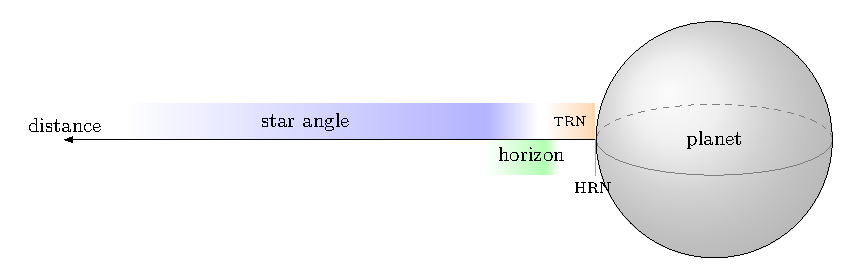
\includegraphics[width=\textwidth]{opnavmethods.pdf}
\caption{\label{fig:opnavmethods}\textbf{A variety of optical navigation methods are able to provide for fully autonomous lunar trajectories.} This diagram corresponds to a roughly logarithmic plot, but is not to scale for the hazard-relative navigation portion of the plot. As an arbitrary example, for a $30^\circ$ field of view camera with a 2,048 pixel focal plane array, horizon navigation is relevant between 65,000 and 6,500 kilometers; and terrain-relative navigation down to around 1--2 kilometers at the equator (based on existing \textsc{lroc} imagery).}
\end{figure}

%While other technologies, such as radars, lidars, and laser altimeters may also provide measurements during descent and landing, there are few other good options for the lunar orbit segment of the trajectory aside from %measurements of stellar occultation by the planet \citep{Keenan1962,Landgraf2006,Psiaki2007,Christian2009} and 
%terrain-relative navigation (\textsc{trn}). % The former provides on the order of a kilometer of error, but can be utilized \citep{Landgraf2006}, and the latter

\subsection{Features for terrain-relative navigation}
The most typical instantiation of terrain-relative navigation, or \textsc{trn}, involves measuring the bearing of surface features of known positions, and provides the flight computer with a few tens or hundreds of meters of position error \citep{Christensen2011}. Terrain features exist at all scales, though the feature catalogue must ultimately be dependent upon the sensor resolution of orbital assets such as the Lunar Reconnaissance Orbiter Camera (about 50 centimeters per pixel) or of landers that have imaged at lower altitudes. A feature catalogue is also limited by registration accuracy, or map tie error, since each feature's position must be estimated with respect to a lunar-fixed frame (which itself includes some error) during catalogue construction.

Craters are a commonly catalogued feature, as reviewed by \citet{Robbins2019}, whose own database includes over one million such features. Such indices are primarily oriented toward planetary geology and other science purposes, however, rather than navigation. Prior to the 2009 launch of the Lunar Reconnaissance Orbiter, they were largely constructed on the basis of imagery, and \citet{Salamuniccar2008} noted substantial registration errors in similarly constructed Martian crater maps. Starting in 2010, the existence of digital terrain models and ready access to far-side imagery generated a rapid increase in catalogue sizes --- but also meant that many craters were identified using non-visual cues. It is also unusual for these databases to include craters smaller than 1 kilometer in diameter. As such, these newer databases are not optimally configured for optical navigation.

Craters are the preferred feature type for most spacecraft terrain-relative navigation needs, due largely to their geometric nature (at least compared to other feature types) and fairly uniform distribution across the lunar surface.

\subsection{Feature detection and matching}
Owing to the different motivations and criteria used by crater detection algorithms, or \textsc{cda}s, there exists no single survey of strategies, and little consensus on the best approach. \citet{Christian2020} have summarized navigation-relevant research, noting that --- as with crater databases --- the goals often differ between scientific and navigation use-cases. Scientific \textsc{cda}s are expected to produce exhaustive lists, whereas for navigation, sensitivity is unimportant, and the goals are speed and sufficient robustness that human supervision is unnecessary. Moreover, many \textsc{cda}s incorrectly assume craters are circular.

While at least one framework has been proposed for comparing the results of different \textsc{cda}s \citep{Salamuniccar2008}, these metrics have not been widely adopted. The lack of adoption may also be driven by the radically different purposes that drive research on these algorithms. The \citet{Salamuniccar2008} framework, for example, offers little assistance with lighting and perspective differences, which are key to our purposes. \citet{Woicke2018} have offered some useful guidance as well as some metrics, but evaluate lighting and perspective robustness only qualitatively. It is thus not straightforward to identify an appropriate \textsc{cda} for our purposes.

Whereas detection aims to locate craters in images, the goal of matching is to link such craters to their entries in catalogues (Figure~\ref{fig:cdma}). \citet{Christian2020} both reviewed crater matching algorithms and identifies an efficient, mathematically rigorous strategy for matching based on invariant theory. They suggest a seven-element descriptor for coplanar craters and a three-element descriptor for non-coplanar craters.

\begin{figure}
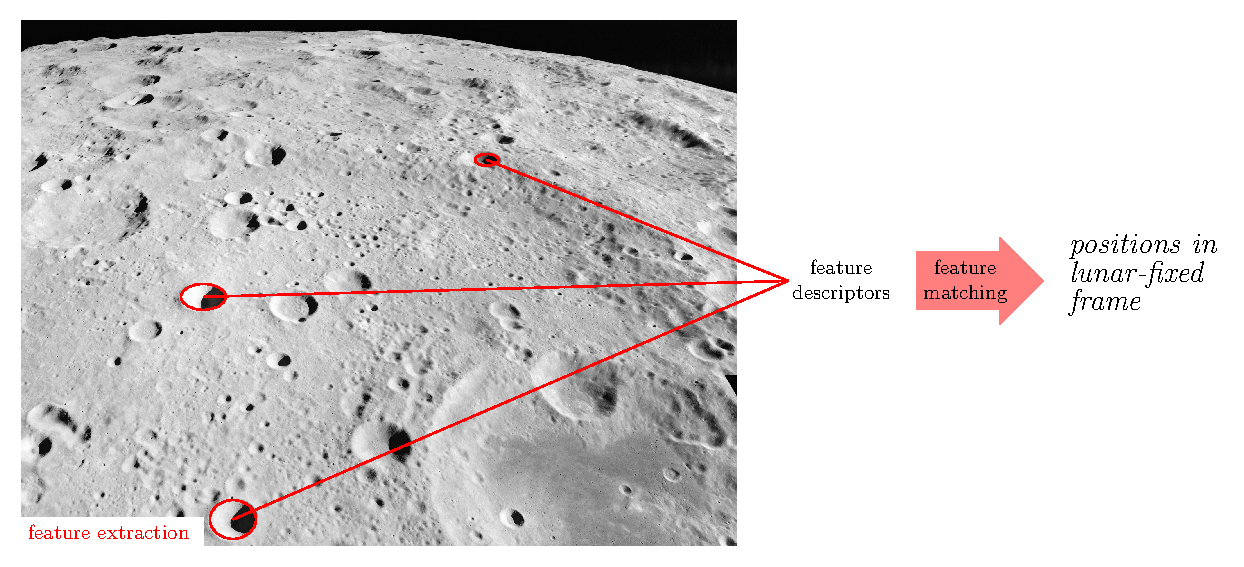
\includegraphics[width=\textwidth]{cdma.pdf}
\caption{\label{fig:cdma}\textbf{Navigation relative to surface features requires algorithms to extract relevant features and to match those features to a catalogue.} Craters are features which are preferred for their relative geometric simplicity, though some craters are substantially more elliptical than others. Even with perfect craters, segmenting out the relevant regions of the image and fitting ellipses to them is a challenging multi-step pattern recognition problem. \citet{Christian2020} have recently demonstrated an elegant approach to the matching component of the problem; patterns of ellipses are represented using descriptors which are viewpoint-invariant, making them easy to store and locate in a database. This image from the Apollo 17 Mapping Camera is courtesy of \textsc{nasa}. }
\end{figure}

With the crater matching aspect largely sewn up, we turn back to crater detection and databases. We know of only one database for crater-based \textsc{trn}. \textsc{Dlr} researchers have constructed an end-to-end crater navigation system, CNav, which demonstrates crater detection and matching, and includes a crater navigation database (which unfortunately is not public) \citep{Maass2016,Maass2020}. Likewise, Intuitive Machines, a Commercial Lunar Payload Services provider, is working on an open source optical navigation system called Thin\textsc{vpu}, which includes a crater detection strategy, but neither a crater matching algorithm nor a database as of yet \citep{Stewart2020}.

Of greater interest to us than a navigation database, however, is the pipeline for producing such a catalogue (Figure~\ref{fig:flowchart}). We expect that the algorithm employed for feature detection in navigation flight software would need to share a great deal of similarity with the algorithm used for database construction --- a common design pattern for feature matching. Because robust feature detection for this purpose is not a solved problem, the production of a navigation feature database alone is insufficient and would suffer from near-term obsolescence. Efforts toward such a pipeline could result in a number of databases, each generated with different extraction algorithms or settings. We might, for example, choose to include an \textsc{orb} or \textsc{sift} feature extractor along with a database of such features.

\subsection{A pipeline and database as a public utility}
A \textsc{gnss} constellation such as \textsc{gps} is at its core a public utility (and hence a public good). For the most part, \textsc{gps} cannot selectively exclude certain users (short of being shut off entirely). Because the \textsc{gps} signal is a broadcast, the system is also non-subtractable (or non-rival); its use by some does not diminish the utility to others.

A pipeline for generating feature databases is likewise a public utility, as are the resulting databases. Their nature as data implies that they are non-excludable and non-subtractable. 

Worth considering is the licensing of such a system. Open source licenses are often classified on a spectrum from restrictive to permissive. The more restrictive \textsc{gnu} General Public License (\textsc{gpl}) 3.0 requires that source code be distributed along with binaries. With more permissive licenses, such as \textsc{mit} or \textsc{bsd}, derivative source code need not be released. The use-case for the software often dictates the license. For example, a commonly used library like Open\textsc{cv} might be released under a permissive license (in this case the \textsc{bsd} 3-clause license) so it can be easily incorporated into commercial products that only use the library incidentally. On the other hand, the Linux kernel is released under a more restrictive license (\textsc{gpl} v2) to ensure that derivative products remain public.

We believe that the proposed pipeline ought to be released under a custom restrictive license with three goals:
\begin{enumerate}
\item Source code for modified pipelines must also be released under a restrictive license.
\item Resulting databases must be made available to the public.
\item The source code for feature extraction algorithms used with the pipeline must be made available to the public.
\end{enumerate}
With appropriate licensing, we can incentivize contribution to a pipeline that may one day provide navigation databases for use on planets other than the Moon, with features that are more efficient to extract than ellipses.

\begin{figure}
\center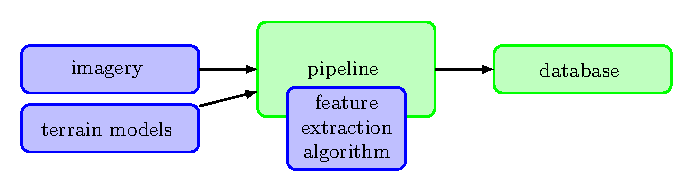
\includegraphics{flowchart.pdf}
\caption{\label{fig:flowchart}\textbf{Our proposed pipeline generates feature databases using a provided feature detection algorithm, planetary imagery, and optional terrain models.} The pipeline itself ought to be licensed under a viral license that also governs the release of the database, regardless of the licensing of the components in blue (imagery, terrain models, and feature algorithm).}
\end{figure}

\section{Research methodology}
\subsection{Crater detection strategies}
The first task is to select an appropriate crater detection algorithm. For initial efforts, we can borrow or modify one from, for example, \citet{Woicke2018}. In the process of building a pipeline, we anticipate --- but hope initially to avoid --- an eventual need to compare the results of various crater detection algorithms under different conditions, namely lighting and viewpoint. To explain why, we must briefly visit the mechanics of image-only \textsc{cda}s, which are sufficiently varied as to be difficult to classify.

Most relevant \textsc{cda}s include a segmentation step, where likely craters are identified within the larger image, and an ellipse-fitting step. Some algorithms, such as those relying on modifications of the Hough transform, are able to perform both steps simultaneously (after performing edge and streak detection).

\citet{Maass2016} helpfully placed segmentation approaches into three categories. Algorithms in the first category aim to identify the crater rims using edge detection strategies. In the second category, methods aim to segment lit or shadowed (or both) areas, which are typically inside of the craters, but sometimes also outside of the crater rims. The third category consists of hybrid approaches. We can add a fourth category for machine learning strategies such as convolutional neural networks \citep{DeLatte2019} and template matching \citep{Bandeira2007}, where the segmentation step is also a classification step. %Some methods also include a pre-segmentation step \citep{Troglio2012}.

\citet{Woicke2018} compared six algorithms --- two which use crater rims, three with high-contrast regions, and one with template matching --- on simulated terrain. They found a great deal of success with segmenting by lit or dark regions, particularly when the illumination direction is known (a problem solved by \citet{Maass2016}). Likewise, \citet{Maass2020} found success with the lit and dark regions.

\textbf{As the high-contrast region segmentation strategy has been met with success in CNav, we intend to use such a method as the baseline for initial pipeline development.}

\subsection{Terrain and imagery}
Our next issue is the identification of useful training data with which to build our database or to test our algorithms.

The Lunar Reconnaissance Orbiter Camera (\textsc{lroc}) team makes available digital terrain models as well as high-resolution imagery (down to 50 cm/px) from the cameras aboard \textsc{lro}. These images, produced by a push-broom rather than pin-hole camera, cannot be used directly in our pipeline without being un-projected and re-projected. Unfortunately, changing the camera model may require additional information about the three-dimensional shape.

\begin{figure}
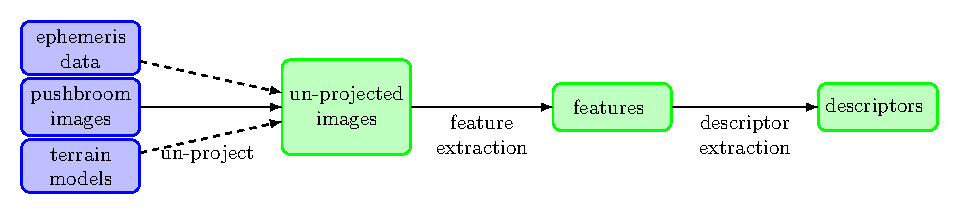
\includegraphics[width=\textwidth]{pipeline.pdf}
\caption{\label{fig:pipeline}\textbf{The pipeline for small-scale features requires generation of a pixel-scale terrain model, in order to transform the wealth of available imagery from the push-broom to the pin-hole camera model.} For larger-scale features, re-projection can be accomplished solely using the published \textsc{lroc} terrain model. Some feature extraction steps, such as for craters, requires an additional descriptor extraction step. This step converts patterns of craters into projective-invariant descriptors which are ultimately stored in the regional indices. These indices make up the full database.}
\end{figure}

For larger-scale terrain features, we plan to rely on the existing \textsc{lroc} digital terrain models, which have a vertical accuracy of 3--4 meters and a horizontal resolution of 60 meters at the equator \citep{Barker2016}. While the error between terrain model tiles is less than the error within a tile, projection of these tiles onto the geoid produces visible seams, particularly in sunlight. These seams represent an as-of-yet unsolved problem that requires further study.

For smaller-scale features, particularly at lower altitudes, the large posting on the the \textsc{lroc dtm} suggests that we can't rely on the terrain models. Fortunately, \textsc{lroc}'s database includes stereo pairs of each narrow angle camera (\textsc{nac}) sweep, and there are many samples of the same terrain under a variety of different lighting conditions. We can likely employ stereo photometry \citep{Woodham1980}, related to photoclinometry (which is often referred to as shape-from-shading) \citep{Horn1977,Kirk1987}, to obtain enough information to re-project the imagery and feed it to our crater detection algorithm.\footnote{An array of techniques including photometric stereo and photoclinometry were recently utilized to produce a pixel-scale digital elevation map of the Moon from \textsc{lroc} narrow angle camera stereo images \citep{Liu2020}. The resulting Chinese digital elevation model is of much higher resolution than the public \textsc{dem} released by the \textsc{lroc} team.}

We expect that image-based crater detection performed on the same terrain under different lighting conditions will produce variations in ellipse parameters, orientation, and location. The \citet{Christian2020} method permits such variation, but we may also wish to employ a modified ellipse fitting strategy which incorporates data from multiple images to produce a consensus crater.

\textbf{The initial iteration of our pipeline may aim to test the crater detection algorithms directly on pushbroom \textsc{lroc} imagery. We plan to improve the pipeline by incorporating a stereo-photometric approach, which will produce a database that meets navigation-level geodetic accuracy requirements} (Figure~\ref{fig:pipeline}).

%These characteristics enable us to turn to an array of photogrammetric techniques that have been developed over the last four decades, which were recently combined to produce a pixel-scale digital elevation model of the lunar surface \citet{Liu2020}. \textit{Photogrammetry} is the measurement of three-dimensional objects (such as point clouds or similar representations) from two-dimensional images. \textit{Photoclinometry}, or shape-from-shading, is a similar technique, which converts pixel intensities into surface gradient information \citep{Horn1977,Kirk1987}. A related technique, which relies on imaging the same object under different illumination directions is termed photometric stereo \citep{Woodham1980}. The resulting maps greatly exceed the resolution of the publicly available \textsc{lroc} models.

\subsection{Crater database}
\citet{Christian2020} proposed the creation of at least two global crater indices, one for non-coplanar craters, and one or more for coplanar crater patterns. It may be useful to produce separate indices for different regions (e.g. using \textsc{Heal}Pix \citep{Gorski2005}) so that, for example, an equatorial mission need not carry polar crater data. We expect to employ a strategy similar to theirs for database construction.

%We plan to use an $n$-dimensional $k$ vector to store the patterns, drawing from experience with star trackers. %We also note the recent demonstration of linear-time star pattern lookups using hash tables consisting of discretized bins to accommodate noisy measurements \citep{Brown2017}. In this method, each of the $k$ star pairs in the pattern can be looked up in $O(1)$ time. We suggest that the same technique may be usable for crater pattern descriptor searches.

Importantly, we intend to generalize the data structures used in the crater database pipeline so that may be used to store descriptors other than the size-3 and size-7 crater pattern invariants.

\section{Conclusion}
We propose the creation of an open source pipeline for generating public lunar navigation feature databases using a variety of feature extraction algorithms. For the initial iteration, we plan to make use of patterns of elliptical craters, which can be described using projection-invariant descriptors.

Our proposal includes steps toward a public digital terrain model of the Moon of significantly higher resolution than the current \textsc{lroc} model. Additionally, it may involve development of photogrammetric techniques particularly useful for the final phase of autonomous lunar landing, hazard-relative navigation, which requires online generation of a three-dimensional map of the intended landing site and its surroundings.

We plan to make all intermediate and final products of our work available to the public under open source licenses, with an eye toward abstraction and maintainability. It is our belief that the resulting products will be useful for a variety of efforts, serving as a navigational public utility until and beyond the eventual introduction of a lunar \textsc{gnss}. Moreover, the pipeline aims to be readily extensible for use on other planets of interest, such as Mars.

Extensibility is a key ingredient for open source projects. In the long term, we envision deploying the pipeline itself aboard future reconnaissance missions. Instead of spending years collecting and painstakingly downlinking image data to Earth, an orbiter equipped with such a toolkit could conceivably generate and downlink a navigation feature database.

\bibliography{craterbase}
\end{document}